% Präambel
\documentclass[12pt,			% Schriftgröße
a4paper,						% Papierformat
twoside, 						% einseitiges (oneside) oder zweiseitiges (twoside) Dokument
listof=totoc, 					% Tabellen- und Abbildungsverzeichnis ins Inhaltsverzeichnis
bibliography=totoc,				% Literaturverzeichnis ins Inhaltsverzeichnis aufnehmen
titlepage, 						% Titlepage-Umgebung statt \maketitle
headsepline, 					% horizontale Linie unter Kolumnentitel
%abstracton,					% Überschrift beim Abstract einschalten, Abstract muss dazu in {abstract}-Umgebung stehen
DIV18,							% auskommentieren, um den Seitenspiegel zu vergrößern
BCOR6mm,						% Bindekorrektur, die den Seitenspiegel um 6mm nach rechts verschiebt,
cleardoublepage=empty,			% Stil einer leeren eingefügten Seite bei Kapitelwechsel
parskip,						% Absatzabstand bei Absatzwechsel einfügen
ngerman							% Übersetzung der festcodierten Überschriften
]{scrbook}			
\usepackage{ucs} 				% Dokument in utf8-Codierung schreiben und speichern
\usepackage{babel} 				% deutsche Trennungsregeln
\usepackage[utf8x]{inputenc} 	% ermöglicht die direkte Eingabe von Umlauten
\usepackage[T1]{fontenc} 		% Ausgabe aller zeichen in einer T1-Codierung (wichtig für die Ausgabe von Umlauten!)
\setlength{\parindent}{0ex} 	% bei neuem Abschnitt nicht einrücken
\linespread{1.2}\selectfont     % Zeilenabstand erhöhen - größere Werte als 1.2 nicht verwenden!!
\usepackage{scrpage2}			% SCR Headings verwenden
\setheadsepline{0.4pt}			% Kopfzeile Linien oben
\setfootsepline{0.4pt}			% Kopfzeile Linien unten
\pagestyle{scrheadings}			% SCR Headings einschalten
\usepackage{graphicx}  			% Einbinden von Grafiken erlauben
\usepackage[format=hang,		% Formatierungen von Unter- / Überschriften
font=normal,
labelfont=bf,
justification=RaggedRight,
singlelinecheck=true,
aboveskip=1mm
]{caption}

\usepackage{enumitem}			% Erlaubt Änderung der Nummerierung in der Umgebung enumerate

\usepackage{amsmath}			% Ergänzungen für Formeln
\usepackage{textcomp} 			% zum Einsatz von Eurozeichen u. a. Symbolen
\usepackage[%
%per=slash,
decimalsymbol=comma,
%thickspace,					
%thickqspace
]{siunitx}						% Einfache Eingabe von SI-Einheiten
\sisetup{number-unit-product = \;, inter-unit-product = \:}
\newcommand*\diff{\mathop{}\!\mathrm{d}}	% Differentialzeichen
\newcommand*\Diff[1]{\mathop{}\!\mathrm{d^#1}} % Differentialzeichen höherer Ableitung
\newcommand*\jj{\mathop{}\!\mathrm{j}}	% Komplexe Zahl j

\usepackage[					% Einstellunge Paket hyperref
hyperfootnotes=false			% im pfd-Output Fußnoten nicht verlinken
]{hyperref}

\usepackage{makeidx}			% Paket zur Erstellung eines Index
\usepackage[printonlyused]{acronym} 	% zur Erstellung des Abkürzungsberzeichnisses

\usepackage[					% Einstellungen für Fußnoten
bottom,							% Ausrichtung unten
multiple,						% Trennung durch Seperator bei mehreren Fußnoten
hang,
marginal
]{footmisc}

\usepackage{calc}				% Paket zum Berechnen von Längen z.B. 0.8\linewidth

\usepackage{xcolor} 			% einfache Verwendung von Farben in nahezu allen Farbmodellen

\usepackage{listings}			% Darstellung von Quellcode mit den Umgebungen {lstlisting}, \lstinline und \lstinputlisting
\lstset{literate=				% Damit können Umlaute innerhalb Listings geschrieben werden
	{Ö}{{\"O}}1
	{Ä}{{\"A}}1
	{Ü}{{\"U}}1
	{ß}{{\ss}}1
	{ü}{{\"u}}1
	{ä}{{\"a}}1
	{ö}{{\"o}}1
}

%****************************************************************** Zusätzliche Packages *******************
%*****************************************************

\usepackage{color}
\usepackage{colortbl}
\usepackage{pdfpages}

%*****************************************************************************************************************************************************************

\definecolor{mygreen}{rgb}{0,0.6,0}
\definecolor{mygray}{rgb}{0.5,0.5,0.5}
\definecolor{mymauve}{rgb}{0.58,0,0.82}
\lstset{ %
	backgroundcolor=\color{white},   % choose the background color; you must add \usepackage{color} or \usepackage{xcolor}; should come as last argument
	basicstyle=\footnotesize,        % the size of the fonts that are used for the code
	breakatwhitespace=false,         % sets if automatic breaks should only happen at whitespace
	breaklines=true,                 % sets automatic line breaking
	captionpos=t,                    % sets the caption-position to (b) bottom or (t) top
	commentstyle=\color{mygreen},    % comment style
	deletekeywords={...},            % if you want to delete keywords from the given language
	escapeinside={\%*}{*)},          % if you want to add LaTeX within your code
	escapeinside={(*@}{@*)},
	extendedchars=true,              % lets you use non-ASCII characters; for 8-bits encodings only, does not work with UTF-8
	frame=none,	                   	% "single" adds a frame around the code; "none"
	keepspaces=true,                 % keeps spaces in text, useful for keeping indentation of code (possibly needs columns=flexible)
	keywordstyle=\color{blue},       % keyword style
	language=[LaTeX]TeX,             % the language of the code
	morekeywords={*,nomenclature},   % if you want to add more keywords to the set
	numbers=left,                    % where to put the line-numbers; possible values are (none, left, right)
	numbersep=5pt,                   % how far the line-numbers are from the code
	numberstyle=\tiny\color{mygray}, % the style that is used for the line-numbers
	rulecolor=\color{black},         % if not set, the frame-color may be changed on line-breaks within not-black text (e.g. comments (green here))
	showspaces=false,                % show spaces everywhere adding particular underscores; it overrides 'showstringspaces'
	showstringspaces=false,          % underline spaces within strings only
	showtabs=false,                  % show tabs within strings adding particular underscores
	stepnumber=1,                    % the step between two line-numbers. If it's 1, each line will be numbered
	stringstyle=\color{mymauve},     % string literal style
	tabsize=2,	                   % sets default tabsize to 2 spaces
	title=\lstname                   % show the filename of files included with \lstinputlisting; also try caption instead of title
}

\makeindex						% Indexverzeichnis erstellen
				% Abkürzungsverzeichnis erstellen

% -----------------------------------------------------------------------------------------------------------------
% Zum Aktualisieren des Abkürzungsverzeichnisses (Nomenklatur) bitte auf der Kommandozeile folgenden Befehl aufrufen :
% makeindex <Dateiname>.nlo -s nomencl.ist -o <Dateiname>.nls
% Oder besser: Kann in TexStudio unter Tools-Benutzer als Shortlink angelegt werden
% Konfiguration unter: Optionen-Erzeugen-Benutzerbefehle: makeindex -s nomencl.ist -t %.nlg -o %.nls %.nlo
% -----------------------------------------------------------------------------------------------------------------

% Hier die persönlichen Daten eingeben:

\newcommand{\titel}{Eintwicklung eines CO2-Messers}
\newcommand{\untertitel}{}
\newcommand{\arbeit}{Mikrocomputertechnik - Bericht}
\newcommand{\studiengang}{Elektrotechnik}
\newcommand{\studienrichtung}{Fahrzeugelektronik}
\newcommand{\autor}{Alexander Herrmann, Johannes Ruffer, Serkant Soylu}
\newcommand{\matrikelnr}{9859538 x 1011921 x 9964027}
\newcommand{\kurs}{TFE18-2}
\newcommand{\abgabe}{19.04.2020}
\newcommand{\zeitraum}{01.10.2019 - 19.04.2020}
\newcommand{\betreuerdhbw}{Hans Jürgen Herpel}
\newcommand{\jahr}{2020}			% für Angabe im Copyright-Vermerk der Titelseite

% Folgende Zeilen definieren Abkürzungen, um Befehle schneller eingeben zu können
\newcommand{\ua}{\mbox{u.\,a.\ }}
\newcommand{\zB}{\mbox{z.\,B.\ }}
\newcommand{\bs}{$\backslash$}

% Folgende Zeilen weden benötigt, um Tikz und PGF-Plot-Grafiken einzubinden
\usepackage{pgfplots}
\usepackage{pgfplotstable}
\pgfplotsset{compat=newest,width=0.6\linewidth}
\usepgfplotslibrary{smithchart}
\usepackage{tikz}						% Tikz sollte nach Listings Pakete geladen werden.
\usetikzlibrary{arrows}
\usetikzlibrary{positioning,shadings}


%\usepackage{pgfkeys,pgfmath,pgfcore}% or pgf or tikz or pgfplots
%
%\pgfkeys{
%	/pgf/number format/textnumber/.style={
%		fixed,
%		use comma,
%		fixed zerofill,
%		precision=4,
%		1000 sep={.},
%	},
%}


\hyphenation{Schrift-ar-ten}

%\renewcommand\thesection{~\arabic{section}}



% -------------------------------------------------------------------------------------------
%                     Beginn des Dokumenteninhalts
% -------------------------------------------------------------------------------------------
\begin{document}
\setcounter{secnumdepth}{3}				% Nummerierungstiefe fürs Inhaltsverzeichnis
\setcounter{tocdepth}{3}
\sffamily								% für die Titelei serifenlose Schrift verwenden

% ------------------------------ Titelei -----------------------------------------------------

\thispagestyle{plain}
\begin{titlepage}
\enlargethispage{4.0cm}
\sffamily 								% Serifenlose Grundschrift für die Titelseite einstellen

\parbox{0.5\linewidth}{
\begin{flushleft}
%\includegraphics[width=0.4\linewidth]{images/Daimler-Logo}\\[5ex]
\end{flushleft}
}
\parbox{0.5\linewidth}{
\begin{flushright}
	
\includegraphics[width=0.4\linewidth]{images/DHBW_d_R_FN_46mm_4c}\\[5ex]
\end{flushright}
}
				

\begin{center}

\LARGE{\textsc{\textbf{\titel}}}\\[1.5ex]
%\Large{\textbf{\untertitel}}\\[5ex]
\Large{\textbf{\arbeit}}\\[2ex]
%\normalsize{für die Prüfung zum\\[1ex] Bachelor of Engineering}\\[3ex]
\Large{Studiengang \studiengang}\\[2ex]
\large{Studienrichtung \studienrichtung}\\[1ex]
\normalsize{Duale Hochschule Baden-Württemberg Ravensburg, Campus Friedrichshafen}\\[5ex]
von\\[1ex] 

\begin{tabular}{ccc}
	& & \\
	Alexander Herrmann & Johannes Ruffer & Serkant Soylu \\
\end{tabular}


\end{center}

\begin{flushleft}

\begin{tabular}{ll}
Abgabedatum:					& \quad \abgabe \\
Bearbeitungszeitraum:		   		& \quad \zeitraum \\ 
Matrikelnummer: 			& \quad \matrikelnr \\
Kurs: 							& \quad \kurs \\
Gutachter der Dualen Hochschule: & \quad \betreuerdhbw \\ [5ex]

\end{tabular} 



\small
%Copyrightvermerk:\\

%Dieses Werk einschließlich seiner Teile ist \textbf{urheberrechtlich geschützt}. Jede Verwertung außerhalb der engen Grenzen des Urheberrechtgesetzes ist ohne Zustimmung des Autors unzulässig und strafbar. Das gilt insbesondere für Vervielfältigungen, Übersetzungen, Mikroverfilmungen sowie die Einspeicherung und Verarbeitung in elektronischen Systemen.
\end{flushleft}
\begin{flushright}
%\copyright{} \jahr
\end{flushright}
\end{titlepage}

\cleardoublepage 				% erzeugt die Titelseite
\pagenumbering{roman}					% kleine, römische Seitenzahlen für Titelei
\chapter*{Eidesstattliche Erklärung} %*-Variante sorgt dafür, das Abstract nicht im Inhaltsverzeichnis auftaucht

%Mit der Abgabe der Aufgabenlösung in Moodle erklären Sie, dass Sie den Programmentwurf selbständig verfasst und keine anderen als die angegebenen Quellen und Hilfsmittel benutzt haben.

Gemäß Ziffer 1.1.13 der Anlage 1 zu §§ 3, 4 und 5  der Studien- und Prüfungsordnung für die Bachelorstudiengänge im Studienbereich Technik der Dualen Hochschule Baden-Würt­tem­berg vom 29.09.2015.

Wir versichern hiermit, dass wir unsere Projektarbeit mit dem Thema: 

\begin{quote}
	\textit{\titel} \textit{ \untertitel }
\end{quote}

selbstständig verfasst und keine anderen als die angegebenen Quellen und Hilfsmittel benutzt haben. Wir versichern zudem, dass die eingereichte elektronische Fassung mit der gedruckten Fassung übereinstimmt.

Friedrichshafen, den \today \\[2ex]

\begin{center}

\begin{tabular}{ccc}
	\rule[-0.2cm]{0.3\linewidth}{0.5pt} & \rule[-0.2cm]{0.3\linewidth}{0.5pt} & \rule[-0.2cm]{0.3\linewidth}{0.5pt}\\
	Alexander Herrmann & Johannes Ruffer & Serkant Soylu\\
\end{tabular}

\rule{0.75\linewidth}{0.1pt}\\
\textsc{Autoren} \\[10ex]
\end{center}


%Sperrvermerk bei Bedarf dekommentieren
%\hrule 
%\vspace*{1.0cm}
%\noindent \textbf{\Large{Sperrvermerk}}\\
%\normalsize
%Die Ergebnisse der Arbeit stehen ausschließlich dem auf dem Deckblatt aufgeführten Ausbildungsbetrieb zur Verfügung.

\normalsize

\rmfamily



\cleardoublepage 				% Einbinden der eidestattlichen Erklärung

\addchap*{Kurzfassung}
% Kurzfassung - Autor:

\label{kurzfassung}

Der Bericht wurde von drei Studierenden an der \ac{DHBW}-Ravensburg Campus Friedrichshafen im Rahmen der Mikrocomputertechnik Vorlesung eigenständig von der Projektplanung, über die Durchführung, bis hin zum Projektabschluss mit Dokumentation durchgeführt. \\
Ziel der Arbeit ist es, durch die Praxiserfahrung mit Mikrocomputern, Fähigkeiten und Wissen in diesem Bereich zu erwerben. Durch das Vergleichen von anfänglichen Kosten- und Komplexitätsschätzungen mit den späteren Ergebnissen in der Umsetzung können die Studierenden ein Fazit ziehen, inwiefern diese übereinstimmen. So werden auch Fähigkeiten im Bereich des Projektmanagements weiterentwickelt. \\
Dieses Projekt befasst sich mit der Simulation eines Fensterhebers. Dabei wird das Öffnen und Schließen der Fenster mithilfe einer \ac{LED} simuliert, welche nach der Überschreitung eines bestimmten Grenzwertes aufleuchtet. Sobald nach ausreichendem Lüften die Luftgüte unter einen Schwellwert gerät, soll die \ac{LED} wieder aus gehen. \\
Damit dies möglich ist, wurde die Entwicklung von Software-Code, sowie ein Schaltungslayout und der 3D-Druck des Gehäuses selbständig vorgenommen. \\
Der folgende Bericht dokumentiert die Motivation, Vorgehensweise und Umsetzung von der Projektplanung, über die Implementierung von Hardware und Software, bis hin zu durchgeführten Tests und dem Projektabschluss.

\tableofcontents						% Erzeugen des Inhalsverzeichnisses
\cleardoublepage

% --------------------------------------------------------------------------------------------
%                    Inhalt der Bachelorarbeit
%---------------------------------------------------------------------------------------------
\pagenumbering{arabic}					% arabische Seitenzahlen für den Hauptteil

\rmfamily

\chapter{Einleitung}
%\setcounter{figure}{0}
\setcounter{chapter}{1}
% Autor:

\label{Einleitung}

Mithilfe eines Arduinos wurde in diesem Projekt ein CO2-gesteuerter Fensterheber simuliert, welcher dazu dienen soll die Räumlichkeiten bei schlechter Luftqualität automatisch zu lüften. Auch das automatische schließen des Fensters nach Wiederherstellung von guter Luftgüte wird simuliert. \\
Das Öffnen und Schließen der Fenster wird anhand von einer LED simuliert, welche nach der Überschreitung eines bestimmten Grenzwertes aufleuchtet. Sobald nach ausreichendem Lüften die Luftgüte unter einen Schwellwert gerät, soll die LED wieder aus gehen. \\
Damit dies möglich ist, wurde die Entwicklung von Software-Code, sowie ein Schaltungslayout und der 3D-Druck des Gehäuses selbständig vorgenommen. \\
Der folgende Bericht dokumentiert die Vorgehensweisen und Umsetzung von der Projektplanung, über die Implementierung von Hardware und Software, bis hin zu durchgeführten Tests und den Projektabschluss.

\chapter{Anforderungen}
\setcounter{chapter}{2}
\label{Anforderungen}

Damit die Bewertung des Projektes erfolgreich wird, müssen zu Projektbeginn Anforderungen erarbeitet und festgelegt werden. Diese sind unveränderbar, da das Ergebnis sonst verfälschen würde.

\begin{table}[!hbt]
	
	\centering
	
	\begin{tabular}{|r| p{8.4cm}|p{4.7cm}|}
		
		\hline
		Nummer & Anforderungen & Verifikationsmethode \\
		\hline
		1 & Echtzeitmessung der Luftgüte & Measurement \\
		\hline
		2 & Mindestmessbereich von 400 ppm bis 5000 ppm & Review \\
		\hline
		3 & Visualisierung der Luftgüte mithilfe von LEDs (gut, mittel, schlecht) & Test \\
		\hline
		4 & Ausgabe der Luftgüte mithilfe von \ac{LCD}-Display & Test \\
		\hline
		5 & Ansteuern eines Fensterscheibenmotors mithilfe einer LED simulieren & Test \\
		\hline
		6 & Bei schlechter Luftgüte: Fenster öffnet sich (LED an) & Test \\
		\hline
		7 & Bei guter Luftgüte: Fenster schließt sich (LED aus) & Test \\
		\hline
		8 & Speichern im CSV-Format & Test, Analysis\\
		\hline
		9 & Zugriff auf Messdaten über SD-Karte & Test \\
		\hline
		10 & Benutzer kann zwischen drei Messprofilen auswählen (Messprofil: Abtastrate) & Test \\
		\hline
		
	\end{tabular}

\captionabove{Anforderungen an das Projekt}
\label{tab:Anforderungen}

\end{table}

Eine Anforderung muss messbar und/oder überprüfbar sein, um deren Umsetzung später objektiv bewerten zu können. Somit wird auch eine sogenannte Verifikationsmethode festgelegt, mit der die Anforderungen später überprüft werden kann. \\
Es gibt sechs verschiedene Verifikationsmethoden:

\begin{itemize}
	\item Similarity: Suche und Abgleich mit bereits vorhandenen Lösungen \cite[S. 122]{HelgaMeyer.}
	\item Insparity: Soll- und Ist-Abgleich von Ein- und Ausgängen nach einem formalen Ablauf (Ein- und Ausgangskriterien sind vorher definiert) \cite[vgl. S. 308]{PeterLiggesmeyer.2009}
	\item Review: Soll- und Ist-Abgleich von Ein- und Ausgängen ohne formalen Ablauf (Ein- und Ausgangskriterien sind vorher nicht definiert) \cite[vgl. S. 317]{PeterLiggesmeyer.2009}
	\item Measurement: Durchführung einer Reihe von Operationen, die das Ziel haben, einen Wert einer quantitativen oder kategorialen Darstellung eines oder mehrerer Attribute zu bestimmen \cite[vgl. S. 395]{DepartmentofResearch&DevelopmentDepartmentofInformationTechnologiesandSystems.}
	\item Analysis: Basiert auf Heuristiken und Statistiken [...] [, die man] sich als starke Compiler-Typisierung [...] im Rahmen einer ausführlichen Datenfluss-Analyse vorstellen [kann] \cite[vgl. S. 4]{JayAbrahamPaulJonesRaoulJetley.}
	\item Test: Prüft und bewertet Software auf Erfüllung der für ihren Einsatz definierten Anforderungen und misst ihre Qualität \cite{Wikipedia.01.03.2020}
\end{itemize}


\chapter{Kostenplan}
\label{KostenundArbeitsplan}

Die Kosten des Projektes belaufen sich, wie in \ref{tab:Kosten} nachzuvollziehen ist, auf 77,13€. An dieser Stelle muss jedoch angefügt werden, dass es sich hierbei nicht um die reinen Materialkosten für das Projekt handelt, da beispielsweise das Arduinoset einiges mehr, als nur die benötigten Materialien geboten hat. Somit kann man sagen, dass sich die Kosten bei einer Bestellung mit Einschränkung auf die benötigten Komponenten senken würden. \\

\begin{table}[!hbt]
	
	\centering
	
	\begin{tabular}{|p{8cm}|p{8cm}|}
		
		\hline
		\rowcolor{lightgray} Einkauf & Kosten \\
		\hline
		Arduinoset & 27,95€ \\
		\hline
		CO2-Sensor (CCS811) & 8,50€ \\
		\hline
		MikroSD-Modul & 3,50€ \\
		\hline
		LED-Fassung & 4,59€ \\
		\hline
		I$^2$C-Adapter & 3,99€ \\
		\hline
		Mechanische Bauteile & 24,99€ \\
		\hline
		Sonstiges & 4,56€ \\
		\hline
		\rowcolor{lightgray} Gesamt & 77,13€ \\
		\hline
		
	\end{tabular}
	
	\captionabove{Aufgewendete Kosten für das Projekt}
	\label{tab:Kosten}
	
\end{table}

\chapter{Arbeitsplan}
\label{Arbeitsplan}


Damit wir zu jedem Zeitpunkt einschätzen können, ob wir im Zeitplan sind, haben wir zu Beginn des Jahres den in Abbildung \ref{fig:Ablaufplan} zu sehenden Projektplan erstellt. An diesen Ablauf inklusive den Daten, hat sich jedes Gruppenmitglied zu halten. Eine Verzögerung in der Entwicklung, bedeutet eine Verschiebung der Abwicklung des Projektes. Davon hängt somit die Fertigstellung, als auch der Erfolg des Projektes ab. \\

\begin{figure}[!hbt]
	\centering
	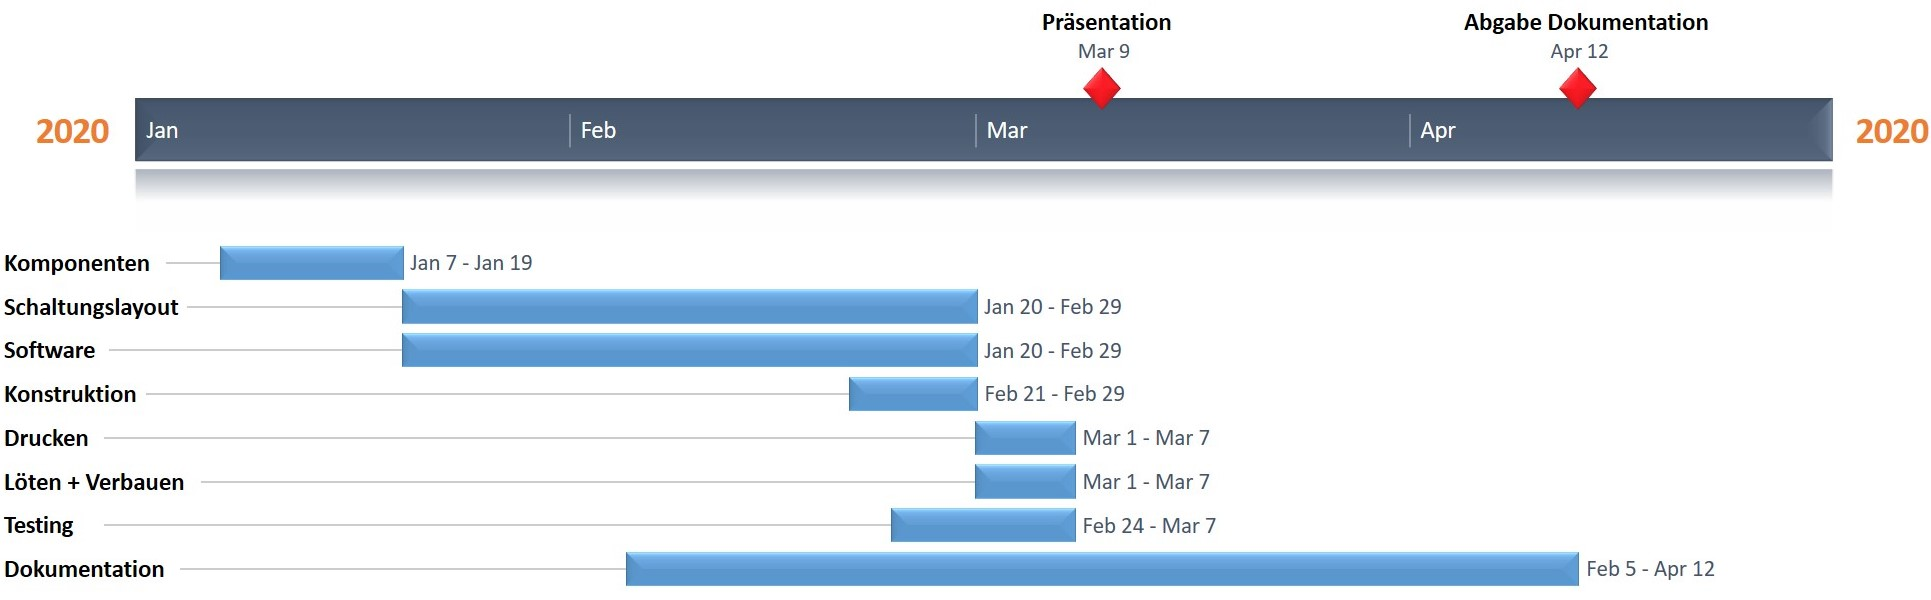
\includegraphics[width=1\linewidth]{Images/Ablaufplan}
	\caption{Ablauf des Projektes von Januar bis April}
	\label{fig:Ablaufplan}
\end{figure}

Auch, wenn die Abgabefrist erst vier Wochen nach Semesterende abläuft, haben wir uns, wie in Abbildung \ref{fig:Ablaufplan} zu sehen ist, den 12. April als Meilenstein für die Abgabe des Projektes gesetzt. Die Begründung für diese Entscheidung liegt zum einen darin, dass wir bei Problemen bezüglich der Abgabe einen gewissen Puffer haben. Zum anderen beginnt ab Anfang April die dritte Praxisphase für alle dualen Studierenden, in welcher diese ab Mitte des Monats schon in ihrem neuen Projekt vertieft sind und somit weniger Zeit für das Mikrocomputertechnik-Projekt aufwenden können.

\chapter{Entwurf}
\label{Entwurf}



\begin{figure}[!hbt]
	\centering
	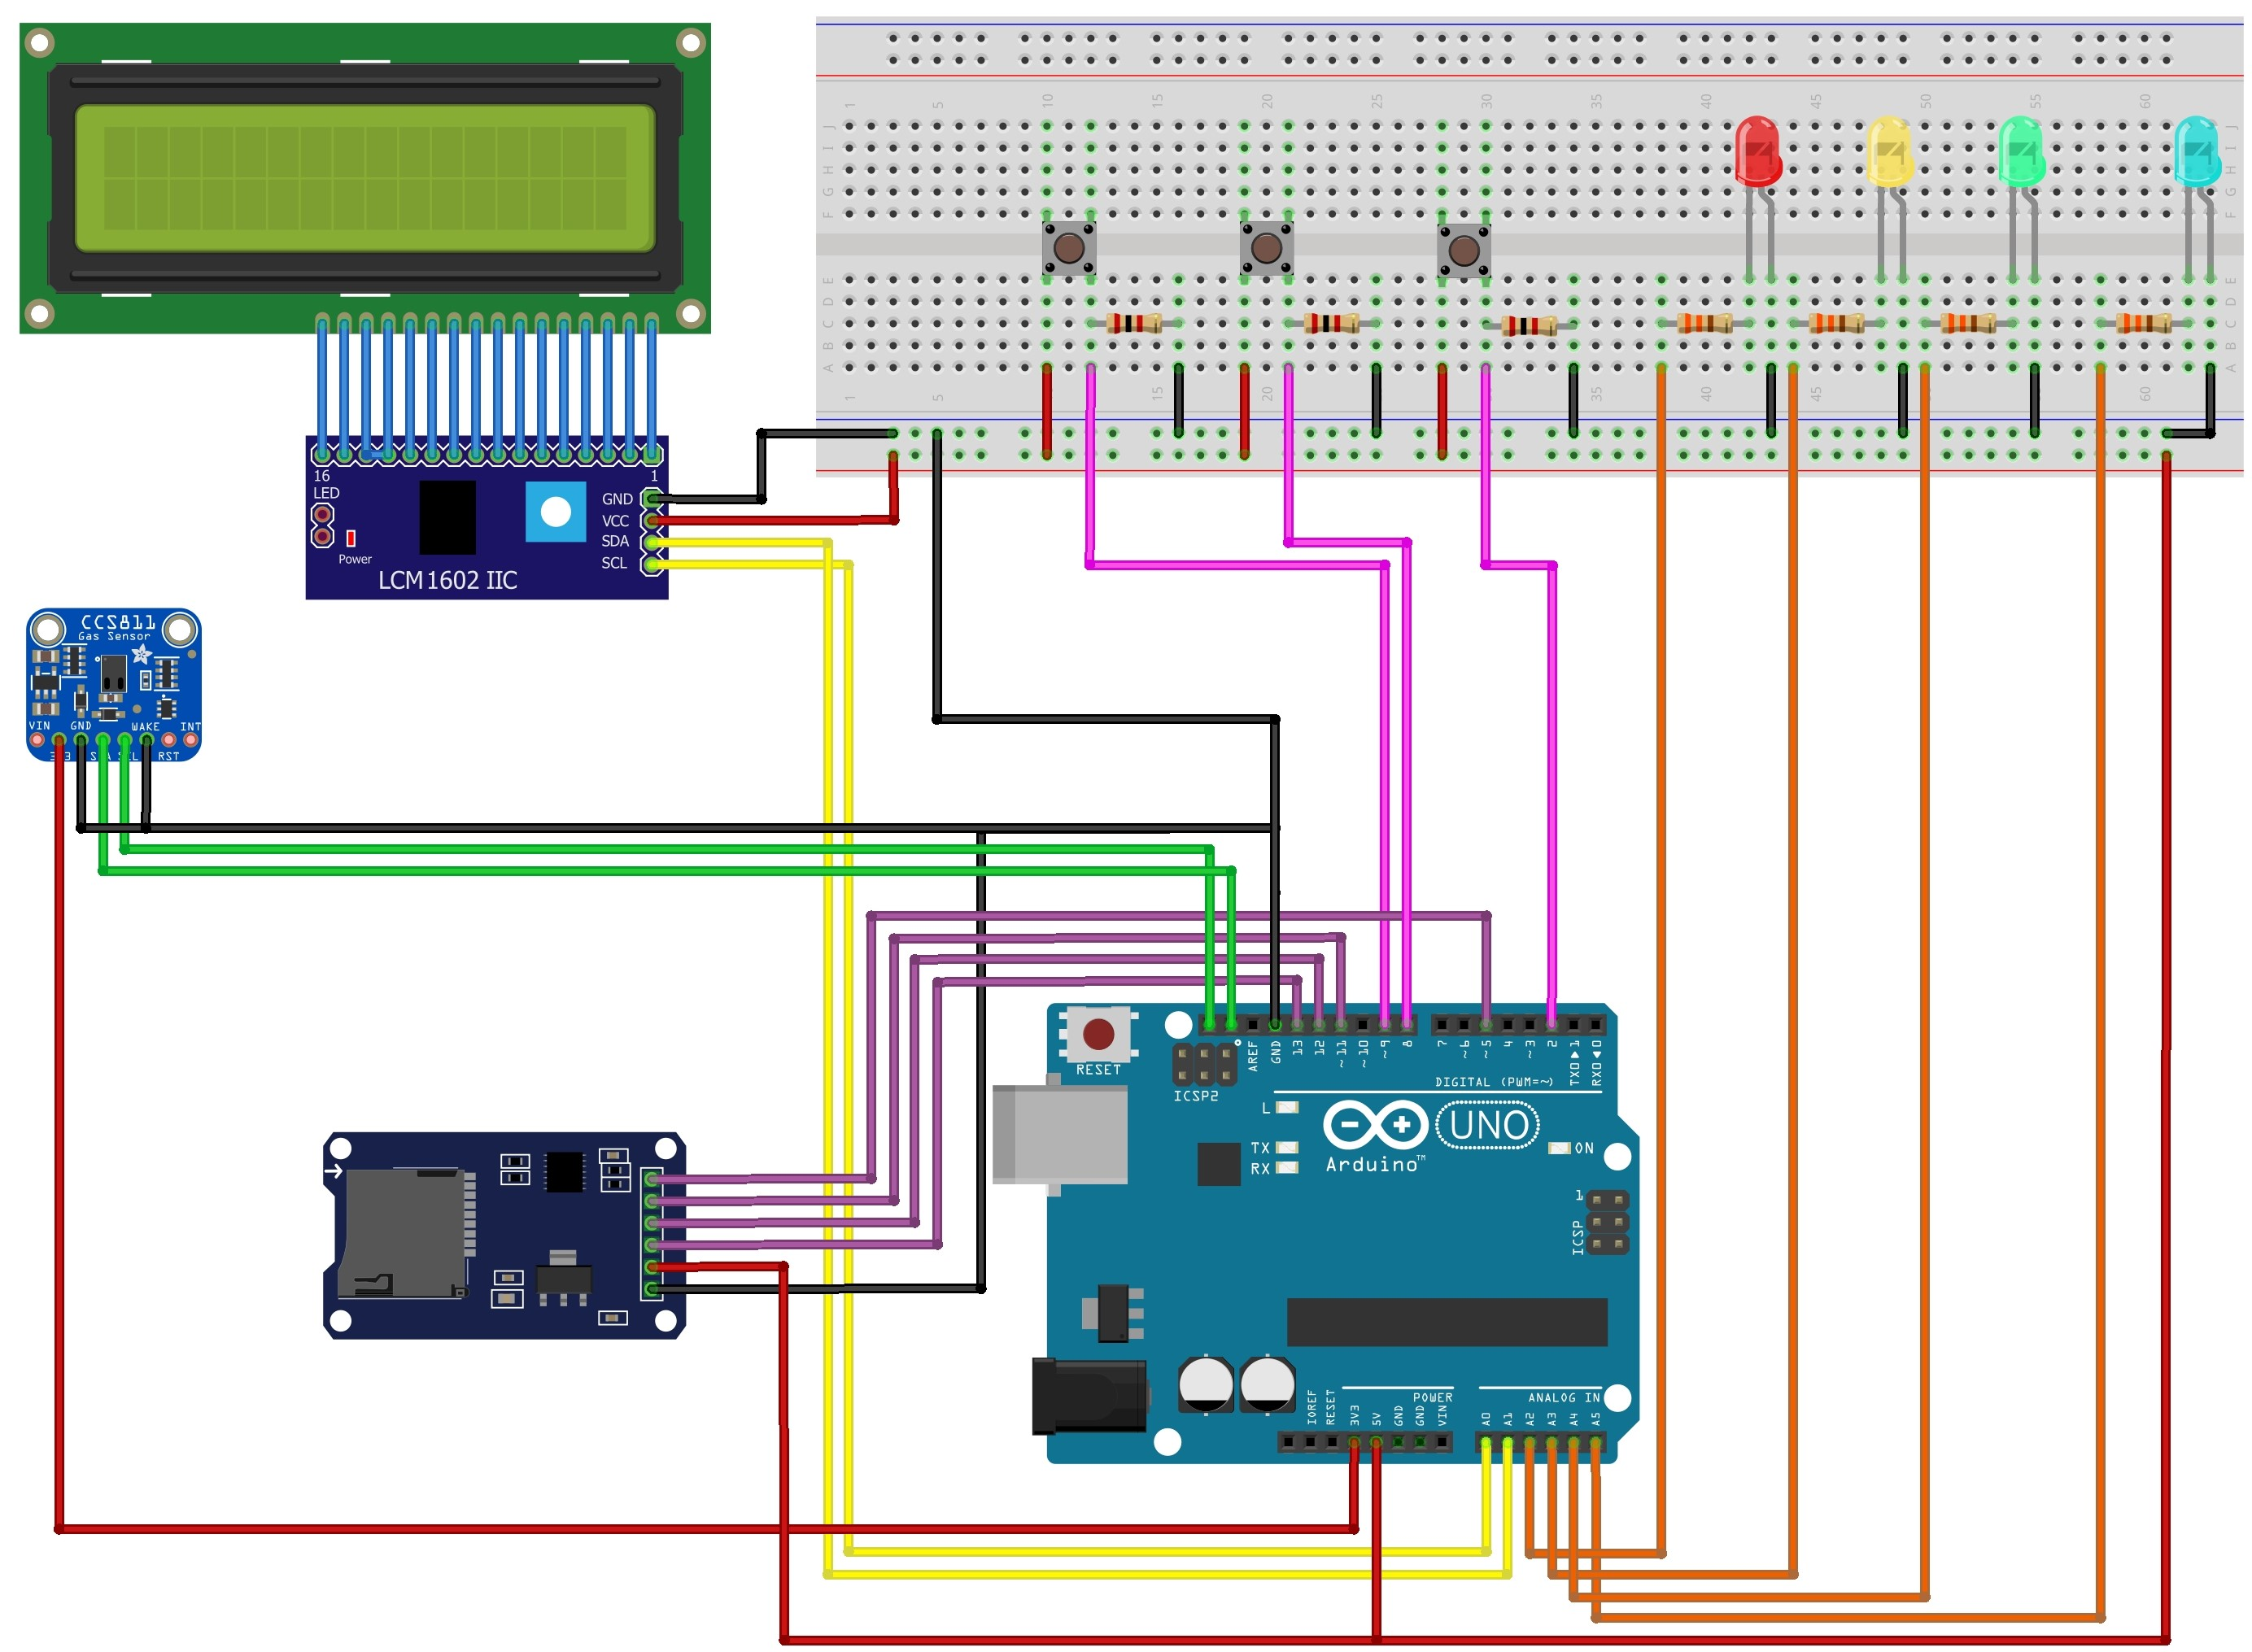
\includegraphics[width=0.9\linewidth]{Images/Layout_Steckplatine}
	\caption{Schaltungslayout vom 27.02.2020}
	\label{fig:Layout}
\end{figure}
\section{Schaltungslayout}
\label{Schaltungslayout}

In Abbildung \ref{fig:Layout} ist das Schaltungslayout des Projektes zu sehen, welches wir mithilfe von Fritzing angefertigt haben. \\
Das \ac{LCD}-Display ist an sechs Pins mit dem Arduino verbunden. Zudem benötigt es eine Versorgungsspannung von ca. 5 Volt. Der Eingang V0 ist dabei über einen Widerstand auf Masse geschalten. Je nach Höhe des Widerstandes ändert sich der Kontrast des \ac{LCD}-Displays. \\
Darunter befindet sich in Abbildung \ref{fig:Layout} der CO2-Sensor CCS811, welcher über zwei Pins an den Arduino angeschlossen ist. Einen extra Anschluss an die Versorgungsspannung benötigt dieser nicht, da er die maximal benötigten $3.6$ Volt über den I$^2$C-Anschluss bekommt. \\
Unterhalb des Co2-Sensors ist das SD-Karten-Modul zu sehen, welches eine Versorgungsspannung von 5 Volt auf Masse benötigt. Die restlichen vier Anschlüsse sind mit den Pins 8 bis 11 am Arduino verbunden. \\
Zwei von den oben zu sehenden Taster dienen für die Menüauswahl auf dem \ac{LCD}-Display. Einer soll dabei für das Wechseln innerhalb des Menüs dienen, der andere ist für die Bestätigung der Auswahl zuständig. Damit die Schaltung auch ein- und ausgeschaltet werden kann, ohne die Versorgungsspannung zu kappen, haben wir einen dritten Taster eingebaut. Die Vorwiderstände aller Taster belaufen sich auf $2\kilo\ohm$. \\
Die vier LEDs sind, wie in den Anforderungen definiert, für die Visualisierung der Luftgüte zuständig. Dabei dienen die Farben Grün, Gelb und Rot für gute, mittlere und schlechte Luftgüte. Die blaue simuliert den angeschlossenen Fensterscheibenmotor. Für die Vorwiderstände der vier LEDs haben wir jeweils $330\ohm$ gewählt. \\

\begin{figure}[!hbt]
	\centering
	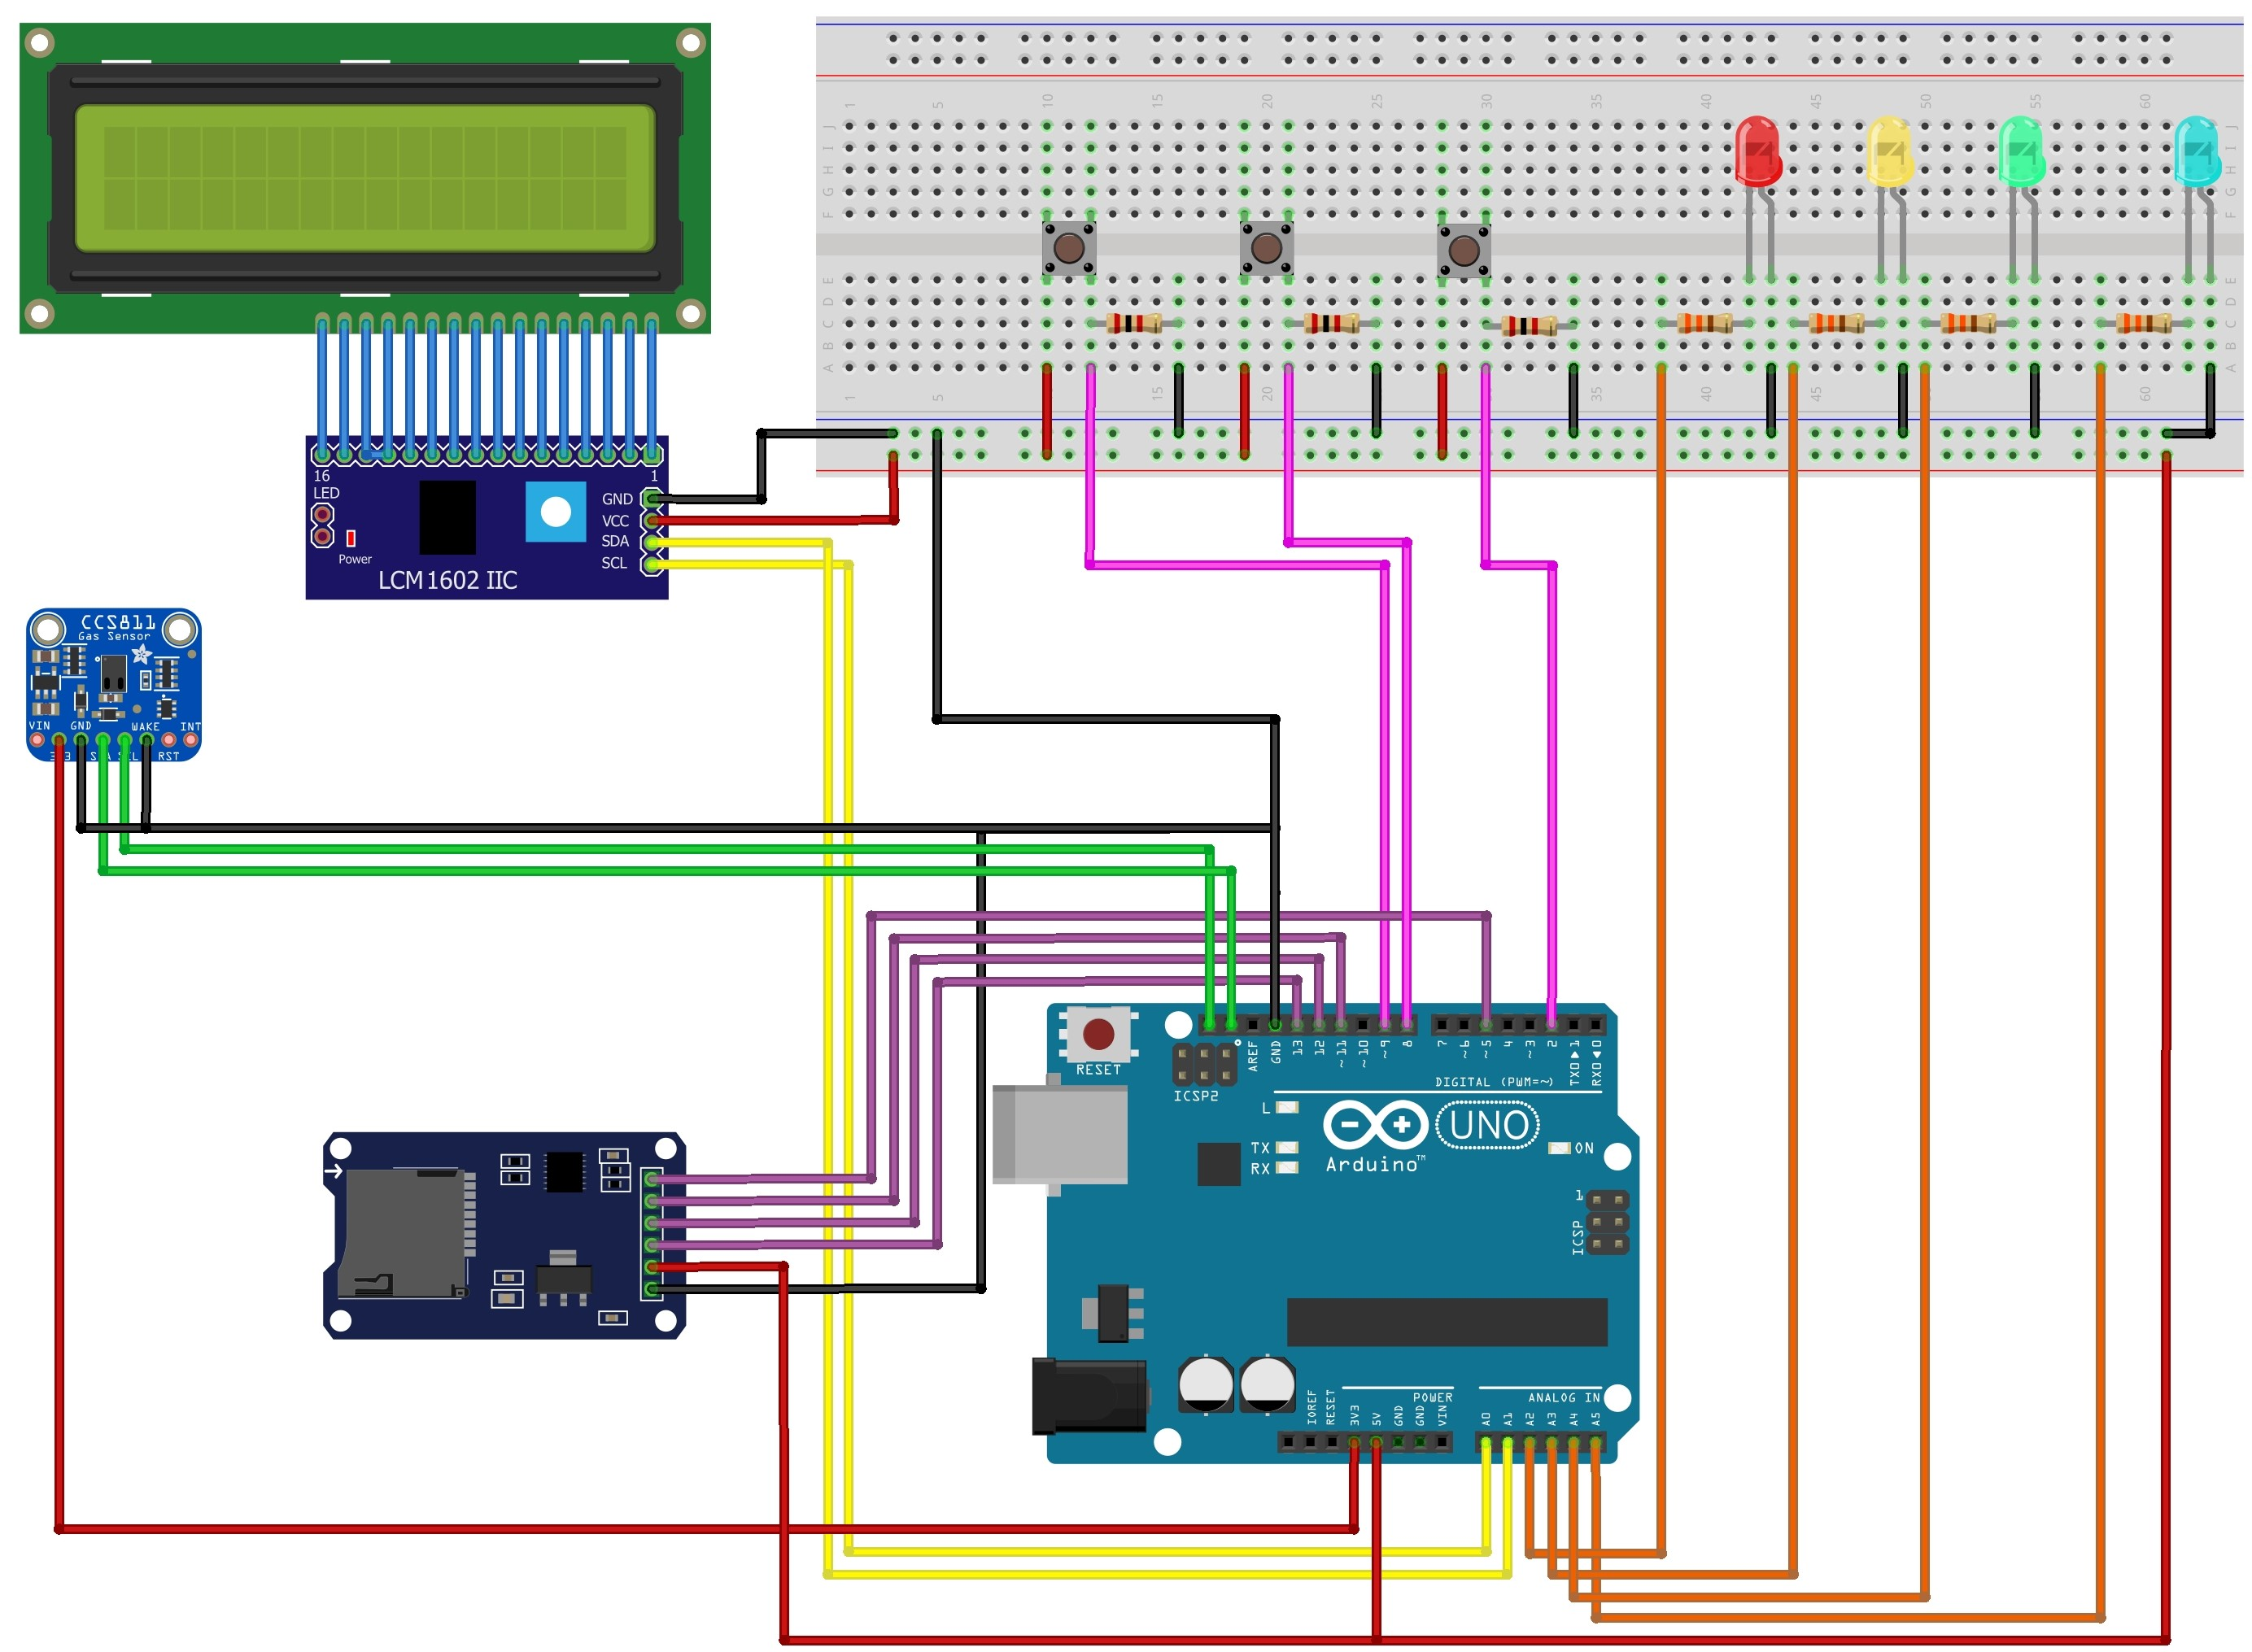
\includegraphics[width=0.9\linewidth]{Images/Layout_Steckplatine}
	\caption{Entwurf des Schaltungslayouts mithilfe von Fritzing}
	\label{fig:Layout}
\end{figure}
\section{Gehäuse}
\input{chapter/Gehäuse}

\chapter{Softwareimplementation}
\label{Softwaremplementation}



Für die entgültige Struktur der Software waren mehrere Anforderungen ausschlaggebend. \\
Zunächst wurden drei verschiedene Messprofile definiert und implementiert, sodass der Benutzer zu Beginn zwischen einer Echtzeit-, Stunden- und Tagesmessung wählen kann. In den Messprofilen ist definiert, in welchen Abständen und wie lange Messungen durchgeführt werden sollen. Somit konnten Anforderung Nummer 1 und 10 aus der Tabelle \ref{tab:Anforderungen} gemeinsam umgesetzt werden. \\
Nach der Wahl des Messprofils muss der Arduino den CO\textsubscript{2}-Sensor ansteuern und richtig konfigurieren. Es muss getestet werden, ob er funktionstüchtig und bereit ist eine Messung zu starten. Zudem kann der verwendete Sensor nicht nur CO\textsubscript{2}-Werte, sondern beispielsweise auch Temperaturen messen, sodass der Arduino die richtigen Werte anfordern muss. Damit dies möglich ist, mussten wir die Bibliothek <Adafruit\_CCS811.h> einbinden. Genaueres zu diesem Algorithmus wird in Kapitel \ref{CCS811} erläutert. \\
Zunächst wird im Setup geprüft, ob der Sensor gestartet werden kann. Falls dies nicht der Fall sein sollte, wird eine Fehlermeldung ausgegeben. Nach erfolgreichem Start ist der Arduino angehalten so lange mit dem Programm zu warten, bis der Sensor zurückmeldet, dass er bereit ist, die Messung zu beginnen. \\
Auch während dem Programmdurchlauf wird bei jeder neuen Messung kontrolliert, ob der CO\textsubscript{2}-Sensor funktionstüchtig ist. Danach wird mithilfe der oben genannten Bibliothek der CO\textsubscript{2}-Wert gemessen und an den Arduino weitergegeben. \\
Nach Einlesen der Daten, vergleicht der Mikrocomputer diese mit den gegebenen Grenzwerten. Je nach Bewertung des gemessenen Werte wird eine der grün/gelb/roten \ac{LED}s eingeschaltet. Auch die blaue \ac{LED}, welche die Ansteuerung des automatisierten Fenstersscheibenmotors simulieren soll, wird je nach Messwert an- oder ausgeschaltet. \\
Zudem werden dem Anwender in Echtzeit die jeweiligen Daten im \ac{LCD} Display aufgegeben, was durch die Bibliothek <LiquidCrystal.h> möglich ist. \\
Damit der Verlauf der Messung später auf Excel geplottet werden kann, wird auf einer Mikro-SD-Karte der gemessene Wert im .csv-Format als .txt-Datei abgespeichert. \\ % Hier noch genauere Ausführung nach fertiger Implementation
Der Anwender nach nun entscheiden, ob er eine weitere Messung durchführen möchte oder nicht. Bei positiver Eingabe wird das Programm von vorne durchgeführt, während beim Ablehnen einer weiteren Messung der Mikrocomputer in einen sogenannten Sleep-Mode geht. % Hier noch genauere Ausführung nach fertiger Implementation




\section{Arduino vs. Raspberry PI}
\label{arduinovsRasbPI}

Nach dem Definieren der Anforderungen musste entschieden werden, mit welchem Mikrocontroller oder auch Einplatinencomputer das Projekt umgesetzt werden soll. Hierbei wurden ein Arduino und ein Raspberry PI in Betracht gezogen. \\
Die Vorteile des Arduinos liegen darin, dass ein sofort einsatzbereites Hardware-/Software-Setup zu Verfügung steht. Des Weiteren hat diser Mikrocontroller eine eigene Entwicklungsumgebung mit plattformübergreifenden Bibliotheken, von welchen wir Gebrauch machen müssen. Zudem ist Arduino eine Plattform, auf Basis von Open-Source-Lizenzen. Dies hat den Vorteil, dass jeder Entwickler sowohl die Quellcodes der Software, als auch die Pläne der Hardware einsehen und für das jeweilige Projekt individuell anpassen kann. \cite[vgl.]{MircoLang.2018} Nachteile, wie die kostspielige Aufrüstung von Shields sind für unsere Verwendungen nicht von Bedeutung. \\
Vielmehr überwiegten die Nachteile des Raspberry PI, für welchen man kostenpflichtige Zusatzteile für den eigenständigen Betrieb benötigt. Auch die Vorteile des Einplatinencomputers, wie die Netzwerkfähigkeit und den standardmäßigen \ac{HDMI}-Anschluss, werden in diesem Projekt nicht benötigt und spielen für uns somit keine Rolle. \cite[vgl.]{IONOS.2018} \\
All diese Punkte führten letztendlich zu der Entscheidung, einen Arduino und keinen Rapberry PI für das Projekt zu nehmen. \\

\section{Arduino}
\label{arduino}

Der Arduino wurde 2005 von den beiden Entwicklern Massimo Banzi und David Cuartielles entwickelt. Der Mikrocomputer wurde nach einer Bar, in welcher sich die Entwickler trafen benannt. Diese wiederum wurde nach Arduin von Ivrea, welcher von 1002 bis 1014 König von Italien war, benannt. \cite[Vgl.]{Wikipedia.2020} \\
Neben 13 digitalen und sechs analogen In- und Output-Pins besitzt der Arduino einen USB-B-Port, mit welchem das Laden eines neuen Programms ermöglicht wird. \\
Die empfohlene Versorgungsspannung liegt hierbei zwischen $7\volt$ und $12\volt$. \cite[Vgl. S. 2]{sertronics.19.03.2020} Er besitzt DC Pins von $5\volt$ und $3,3\volt$ DC-Spannung. \\


\section{CCS811}
\label{CCS811}

Wir haben den in Abbildung \ref{fig:CCS811-Bild}  zu sehenden CCS811-Sensor verwendet da er einige Vorteile mit sich bringt. Er ist ein digitaler \ac{MOX}-Gassensor mit einem extrem geringen Stromverbrauch. Wie in Abbildung \ref{fig:ccs811Blockdiagramm} zu sehen ist, besitzt er einen \ac{AD}-Wander und eine I$^2$C-Schnittstelle, was dem Entwickler eine leichte Soft- und Hardware Integration bietet. Zudem soll er eine Lebenszeit von über 5 Jahren nachweisen. \cite[vgl. S. 1]{amsAG.2016} \\

\begin{figure}[!hbt]
	\centering
	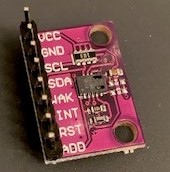
\includegraphics[width=0.3\linewidth]{Images/CO2SensorCCS811}
	\footnotesize \\Quelle: eigene Aufnahme
	\caption{Verwendeter CCS811-\ac{MOX}-Gassensor}
	\label{fig:CCS811-Bild}
\end{figure}

Der CO2-Sensor ist über die Pins SDA und SCL mit dem Arduino verbunden. Pin 7 ist dabei auf Masse kurzgeschlossen. Die restlichen Pins werden in unserem Projekt nicht benötigt.

\begin{figure}[!hbt]
	\centering
	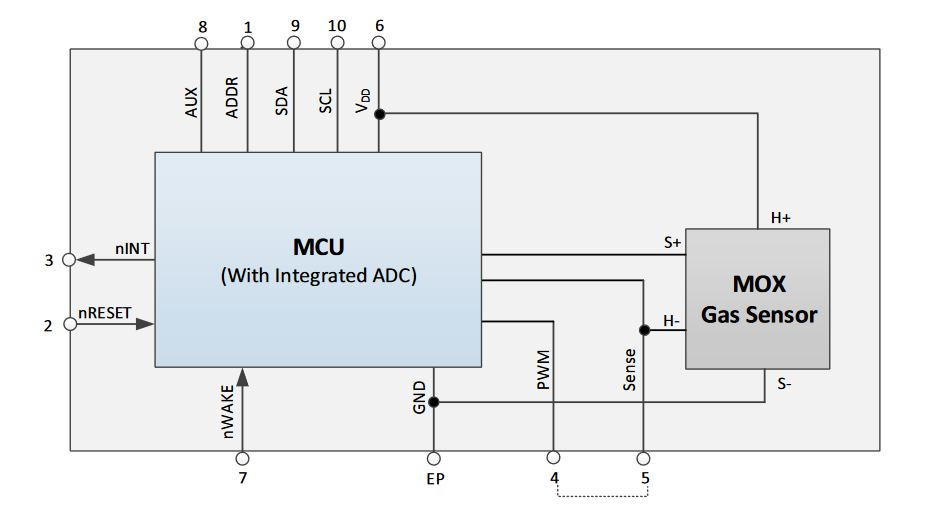
\includegraphics[width=0.8\linewidth]{Images/ccs811Blockdiagramm}
	\footnotesize{\\ Quelle: \cite[S. 3]{amsAG.2016}}
	\caption{Komponentendiagramm des CCS811}
	\label{fig:ccs811Blockdiagramm}
\end{figure}

Der Abruf von Messdaten auf dem I$^2$C erfolgt über das Master-Slave Prinzip. Dabei nimmt der Arduino die Rolle des Masters, und der CO\textsubscript{2}-Sensor die des Slaves ein. Das bedeutet, der CCS811 darf nur Informationen senden, wenn er vom Arduino die Aufforderung bekommen hat. \\
Um an die richtigen Daten des Sensors zu gelangen, muss der Arduino in unserem Projekt die ersten beiden Bytes auslesen, da diese die nötigen Informationen über den CO\textsubscript{2}-Gehalt der Luft zu Verfügung stellen. Die restlichen Bytes werden in unserem Projekt nicht ausgelesen, da wir für diese keine Verwendung haben.
\begin{center}
	\begin{figure}[!hbt]
		\centering
		\begin{tikzpicture}[scale=0.9]
		
		% Gitter zeichnen (spalte zeile)
		\draw (1,0)--(17,0); 
		\draw (1,1)--(17,1); 
		\draw (1,2)--(17,2);
		
		\draw (1,3)--(17,3);
		\draw (1,4)--(17,4);
		\draw (1,5)--(17,5);
		
		\draw (1,3)--(1,5)node [right,near end]{Byte 0} node[right,near start]{eCO\textsubscript{2} High Byte}; % linke Linie Slave Adress
		\draw (5,3)--(5,5)node [right,near end]{Byte 1} node[right,near start]{eCO\textsubscript{2} Low Byte}; % linke Linie W
		\draw (9,3)--(9,5)node [right,near end]{Byte 2} node[right,near start]{TVOC High Byte};
		\draw (13,3)--(13,5)node [right,near end]{Byte 3} node[right,near start]{TVOC Low Byte};
		\draw (17,3)--(17,5);
		
		\draw (1,0)--(1,2)node [right,near end]{Byte 4} node[right,near start]{STATUS};
		\draw (5,0)--(5,2)node [right,near end]{Byte 5} node[right,near start]{ERROR\_ID};
		\draw (9,0)--(9,2)node [right,near end]{Byte 6} node[right,near start]{See RAW\_DATA};
		\draw (13,0)--(13,2)node [right,near end]{Byte 7} node[right,near start]{See RAW\_DATA};
		\draw (17,0)--(17,2);
				
		\end{tikzpicture}
		\footnotesize{\\Quelle: \cite[vgl. S. 14]{amsAG.2016}}
		\caption{Inhalt der 8-Byte-Übertragung des CCS811-\ac{MOX}-Sensors}
		\label{fig:8ByteInfo}
	\end{figure}
\end{center}
In der Softwareimplementierung wird der Co\textsubscript{2}-Sensor mithilfe der Bibliothek <Ardafruit\_CCS811.h>, wie in Abbildung \ref{fig:Setup} gezeigt wird, aufgerufen. Zunächst werden Setups für das I$^2$C-Interface und die Hardware durchgeführt. Danach wird geprüft, ob die Kommunikation mit dem Sensor aufgebaut werden kann. Wenn das der Fall ist, wird solange gewartet, bis der Sensor bereit ist, Daten zu lesen. Falls jedoch ein Problem auftritt, wird eine Fehlermeldung ausgegeben und der Arduino geht in eine sogenannte Endlosschleife, bis das Programm neu geladen oder der Arduino ausgeschalten wird.

\begin{figure}[!hbt]
	\centering
	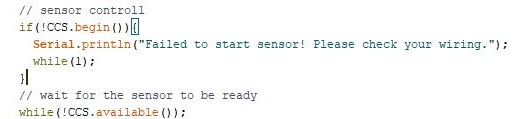
\includegraphics[width=0.8\linewidth]{Images/ccs811Setup}
	\caption{Codeausschnitt zur Sensor-Kontrolle im aus dem Quellcode}
	\label{fig:Setup}
\end{figure}

Die Abfrage der CO\textsubscript{2}-Werten erfolgt über eine weitere Prüfung auf Fehler und einer darauffolgenden Messung. Das in Array dient hierbei zur Zwischenspeicherung der Daten. Anschließend werden die gespeicherten Informationen an die Mikro-SD-Karte weitergegeben. Näheres dazu in Kapitel \ref{microSD}.

\begin{figure}[!hbt]
	\centering
	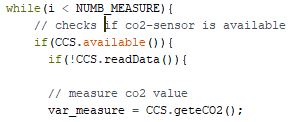
\includegraphics[width=0.5\linewidth]{Images/ccs811Loop}
	\caption{Codeausschnitt für die Messung aus dem Quellcode}
	\label{fig:Loop}
\end{figure}



\section{Mikro-SD}
\label{microSD}

Zunächst sollten die gemessenen CO$_2$-Werte auf dem Arduino selbst abgespeichert werden. Der EEPROM wäre dafür die Lösung gewesen. Jedoch besitzt dieser eine Speicherkapazität von 1KB. Bei größeren Messungen reicht das unter Umständen nicht aus, sodass eine Methode gefunden werden musste, in welcher die Daten extern vom Arduino abgespeichert werden können. \\
Dazu haben wir den, in Abbildung \ref{fig:SD-Modul} zu sehenden Mikro-SD-Karten-Adapter hinzugezogen. Hier können die gemessenen CO$_2$-Werte ohne Speicherprobleme gesichert werden. \\

\begin{figure}[!hbt]
	\centering
	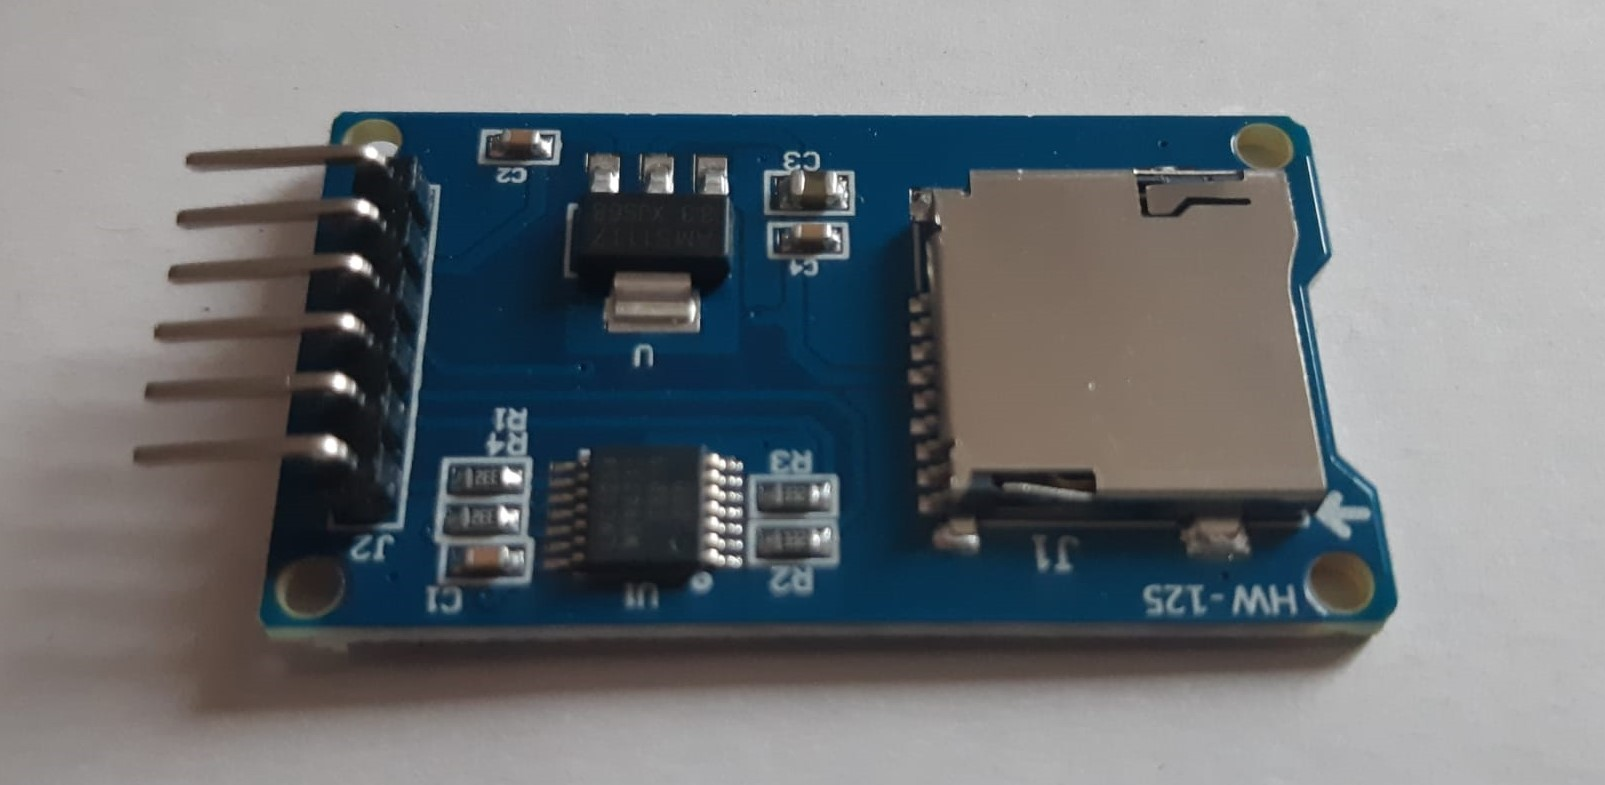
\includegraphics[width=0.7\linewidth]{Images/Mikro-SD_2}
	\footnotesize{\\ Quelle: eigene Aufnahme}
	\caption{Verwendeter Mikro-SD-Karten-Adapter, mit Sicht auf dessen Vorderseite}
	\label{fig:SD-Modul}
\end{figure}

Der Mikro-SD-Karten-Adapter ist über die, in Abbildung \ref{fig:SD-Modul_RUCK} zu sehenden PINs MISO, MOSI, SCK und CS, mit dem Arduino verbunden. Die komplementären PINs des Arduinos sind in Abbildung \ref{fig:Layout} zu sehen. Der Adapter benötigt zudem eine Versorgungsspannung von mindestens $4,5\volt$ bis maximal $5,5\volt$ zur Masse. \cite[vgl. S. 1]{ebaySearch.} \\

\begin{figure}[!hbt]
	\centering
	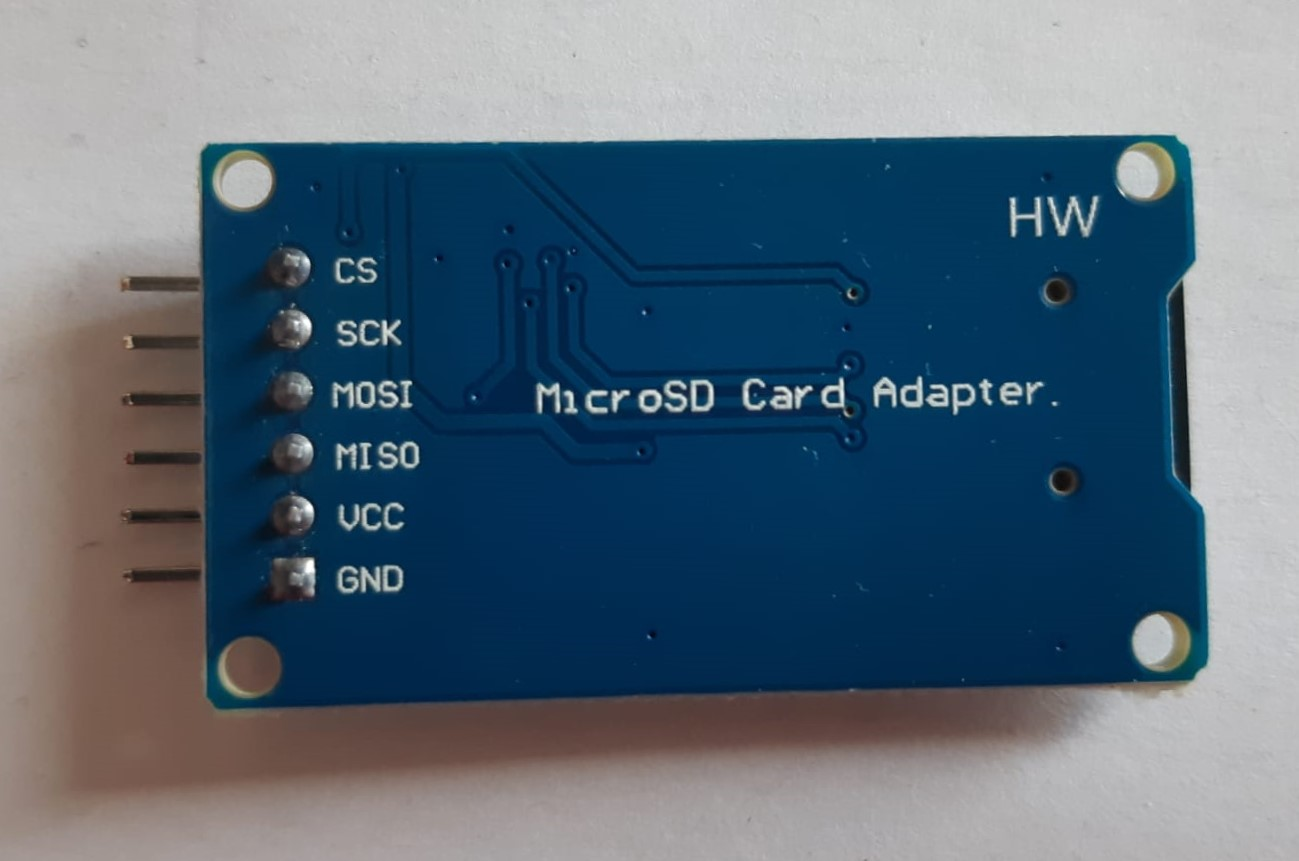
\includegraphics[width=0.6\linewidth]{Images/Mikro-SD_3}
	\footnotesize{\\ Quelle: eigene Aufnahme}
	\caption{Verwendeter Mikro-SD-Karten-Adapter, mit Sicht auf dessen Rückseite}
	\label{fig:SD-Modul_RUCK}
\end{figure}

Für die Integration der SD-Karte, muss zunächst die Bibliothek <SD.h> eingebunden werden. Anschließend wird eine globale Variable als File deklariert. In unserem Programmablauf wird die anschließende Initialisierung der SD-Karte zweimal durchgeführt. Das erste mal im Setup, vor dem Programmablauf. Die Begründung liegt darin, dass dem Benutzer bei fehlender SD-Karte schon vor der Auswahl des Messmodus eine Fehlermeldung angezeigt werden kann. Das zweite Mal wird die SD-Karte vor dem Start der Messung durchgeführt. Das hat den Hintergrund, dass die SD-Karte kurz davor entfernt werden könnte. Auch hier wird bei fehlender Karte der Benutzer durch eine Ausgabe informiert. Zudem wird das Programm anschließend neu gestartet. \\
Vor dem Start der Messung wird außerdem eine .txt-Datei auf der SD-Karte erstellt. Im Fall, dass eine gleichnamige Textdatei bereits existiert, wird diese zum schreiben geöffnet. An dieser Stelle wird im Programmcode auch definiert, dass der Arduino die SD-Karte beschreiben und nicht auslesen soll. \\
Während der Messung bleibt die SD-Karte geöffnet und der Arduino im Schreibe-Modus, sodass kein lokaler Speicher für die Übertragung der Daten benötigt wird. Somit können so viele Messungen durchgeführt werden, wie Speicherkapazität auf der SD-Karte vorhanden ist. Nach Beenden der Messung wird die Textdatei abgespeichert und geschlossen. \\

\begin{figure}[!hbt]
	\centering
	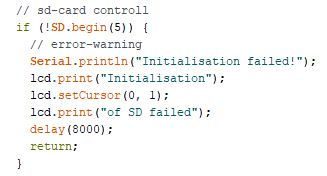
\includegraphics[width=0.6\linewidth]{Images/sdSetup}
	\footnotesize{\\ Quelle: eigene Aufnahme}
	\caption{Codeausschnitt zur Initialisierung der SD-Karte im Setup aus dem Quellcode}
	\label{fig:SD_Setup}
\end{figure}



\chapter{Hardware}
\label{Projektbeschreibung}




\chapter{Testing}
\label{Testing}

\begin{table}[!hbt]
	
	\centering
	
	\begin{tabular}{|p{5cm}|p{5cm}|}
		
		\hline
		Projekt: CO2-Sensor & Datum: \\
		\hline
		ID: CO201 & Version: 1.0 \\
		\hline
		\multicolumn{2}{|l|}{Titel: Visualisierung der Luftqualität auf Basis von CO2-Grenzen} \\
		\hline
		Items: void ask(int) & TestKfg: 01 \\
		\hline
		\multicolumn{2}{|p{\textwidth-2\tabcolsep}|}{Zielsetzung: Der Test soll zeigen, dass die Software die gemessenen CO2-Werte richtig interpretieren kann.} \\
		\hline
		\multicolumn{2}{|l|}{Anforderungen: R01} \\
		\hline
		\multicolumn{2}{|l|}{Erforderliche Inputs zu Testbeginn: CO2 Werte} \\
		\hline
			
	\end{tabular}

\captionabove{Test 1}
\label{tab:Test_1}

\end{table}

\begin{table}[!hbt]
	
	\centering
	
	\begin{tabular}{|p{7.4cm}|p{7.4cm}|}
	
		\hline
		Tester: & Beobachter: \\
		\hline
		\multicolumn{2}{|l|}{Protokolldatei: } \\
		\hline
		Status: & Problembericht: \\
		\hline
	
	\end{tabular}

	\captionabove{Tester 1}
	\label{tab:Tester1}

\end{table}


\begin{table}[!hbt]
	
	\centering
	
	\begin{tabular}{|p{5cm}|p{5cm}|}
		
		\hline
		Projekt: CO2-Sensor & Datum: \\
		\hline
		ID: CO202 & Version: 1.0 \\
		\hline
		\multicolumn{2}{|l|}{Titel: Auswahl von verschiedenen Messprofilen} \\
		\hline
		Items: void ask(int) & TestKfg: 01 \\
		\hline
		\multicolumn{2}{|p{\textwidth-2\tabcolsep}|}{Zielsetzung: Der Test soll zeigen, dass der Anwender zwischen drei verschiedenen Messprofilen wählen kann.} \\
		\hline
		\multicolumn{2}{|l|}{Anforderungen: R03} \\
		\hline
		\multicolumn{2}{|l|}{Erforderliche Inputs zu Testbeginn: Anwender} \\
		\hline
		
	\end{tabular}
	
	\captionabove{Test 2}
	\label{tab:Test_2}
	
\end{table}

\begin{table}[!hbt]
	
	\centering
	
	\begin{tabular}{|p{8cm}|p{8cm}|}
		
		\hline
		Tester: Alexander Herrmann & Beobachter: Johannes Ruffer \\
		\hline
		\multicolumn{2}{|l|}{Protokoll: Zunächst wurde der Arduino an den Laptop angeschlossen und somit das aktuelle Programm gestartet. } \\	\hline
		Status: Erfolgreich & Problembericht: Nicht vorhanden \\
		\hline
		
	\end{tabular}
	
	\captionabove{Tester 2}
	\label{tab:Tester2}
	
\end{table}



\chapter{Handbuch}
\label{Handbuch}

\chapter{Installationsanleitung}
\label{Installationsanleitung}

Nachfolgend finden Sie eine Anleitung, wie Sie den CO$_2$-Messer in Betrieb nehmen. Bitte beachten Sie auch die zusätzlichen Hinweise. \\
Damit die Software erfolgreich vom Computer auf den Arduino geladen werden kann, müssen die folgenden Bibliotheken heruntergeladen sein:

\begin{itemize}
	\item Adafruit\_CCS811.h (Arduino-Driver für den CCS811 Gas-Sensor)
	\item SPI.h (Ermöglicht die Kommunikation mit dem Serial Peripheral Interface)
	\item Wire.h (Ermöglicht die Kommunikation über $I^2C$)
	\item LiquidCrystal.h (Zur Integration des \ac{LCD}-Displays)
	\item SD.h (Ermöglicht die Kommunikation mit dem Mikro-SD-Karten-Adapter)
\end{itemize}

\begin{figure}[!hbt]
	\centering
	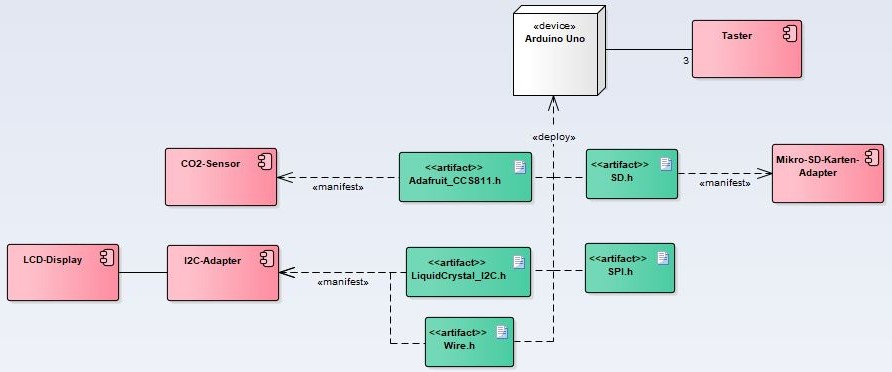
\includegraphics[width=0.9\linewidth]{Images/Diploymentdiagramm}
	\footnotesize \\Quelle: eigene Aufnahme
	\caption{Diploymentdiagramm zum Verständnis der Integration von Soft- und Hardware und deren Verbindungen}
	\label{fig:Diployment}
\end{figure}

Zunächst muss der I$^2$C-Adapter, wie in Abbildung \ref{fig:I2C} abgebildet ist, an das \ac{LCD}-Display angeschlossen werden. Achten Sie auf die Richtung der beiden Elemente. \\

\begin{figure}[!hbt]
	\centering
	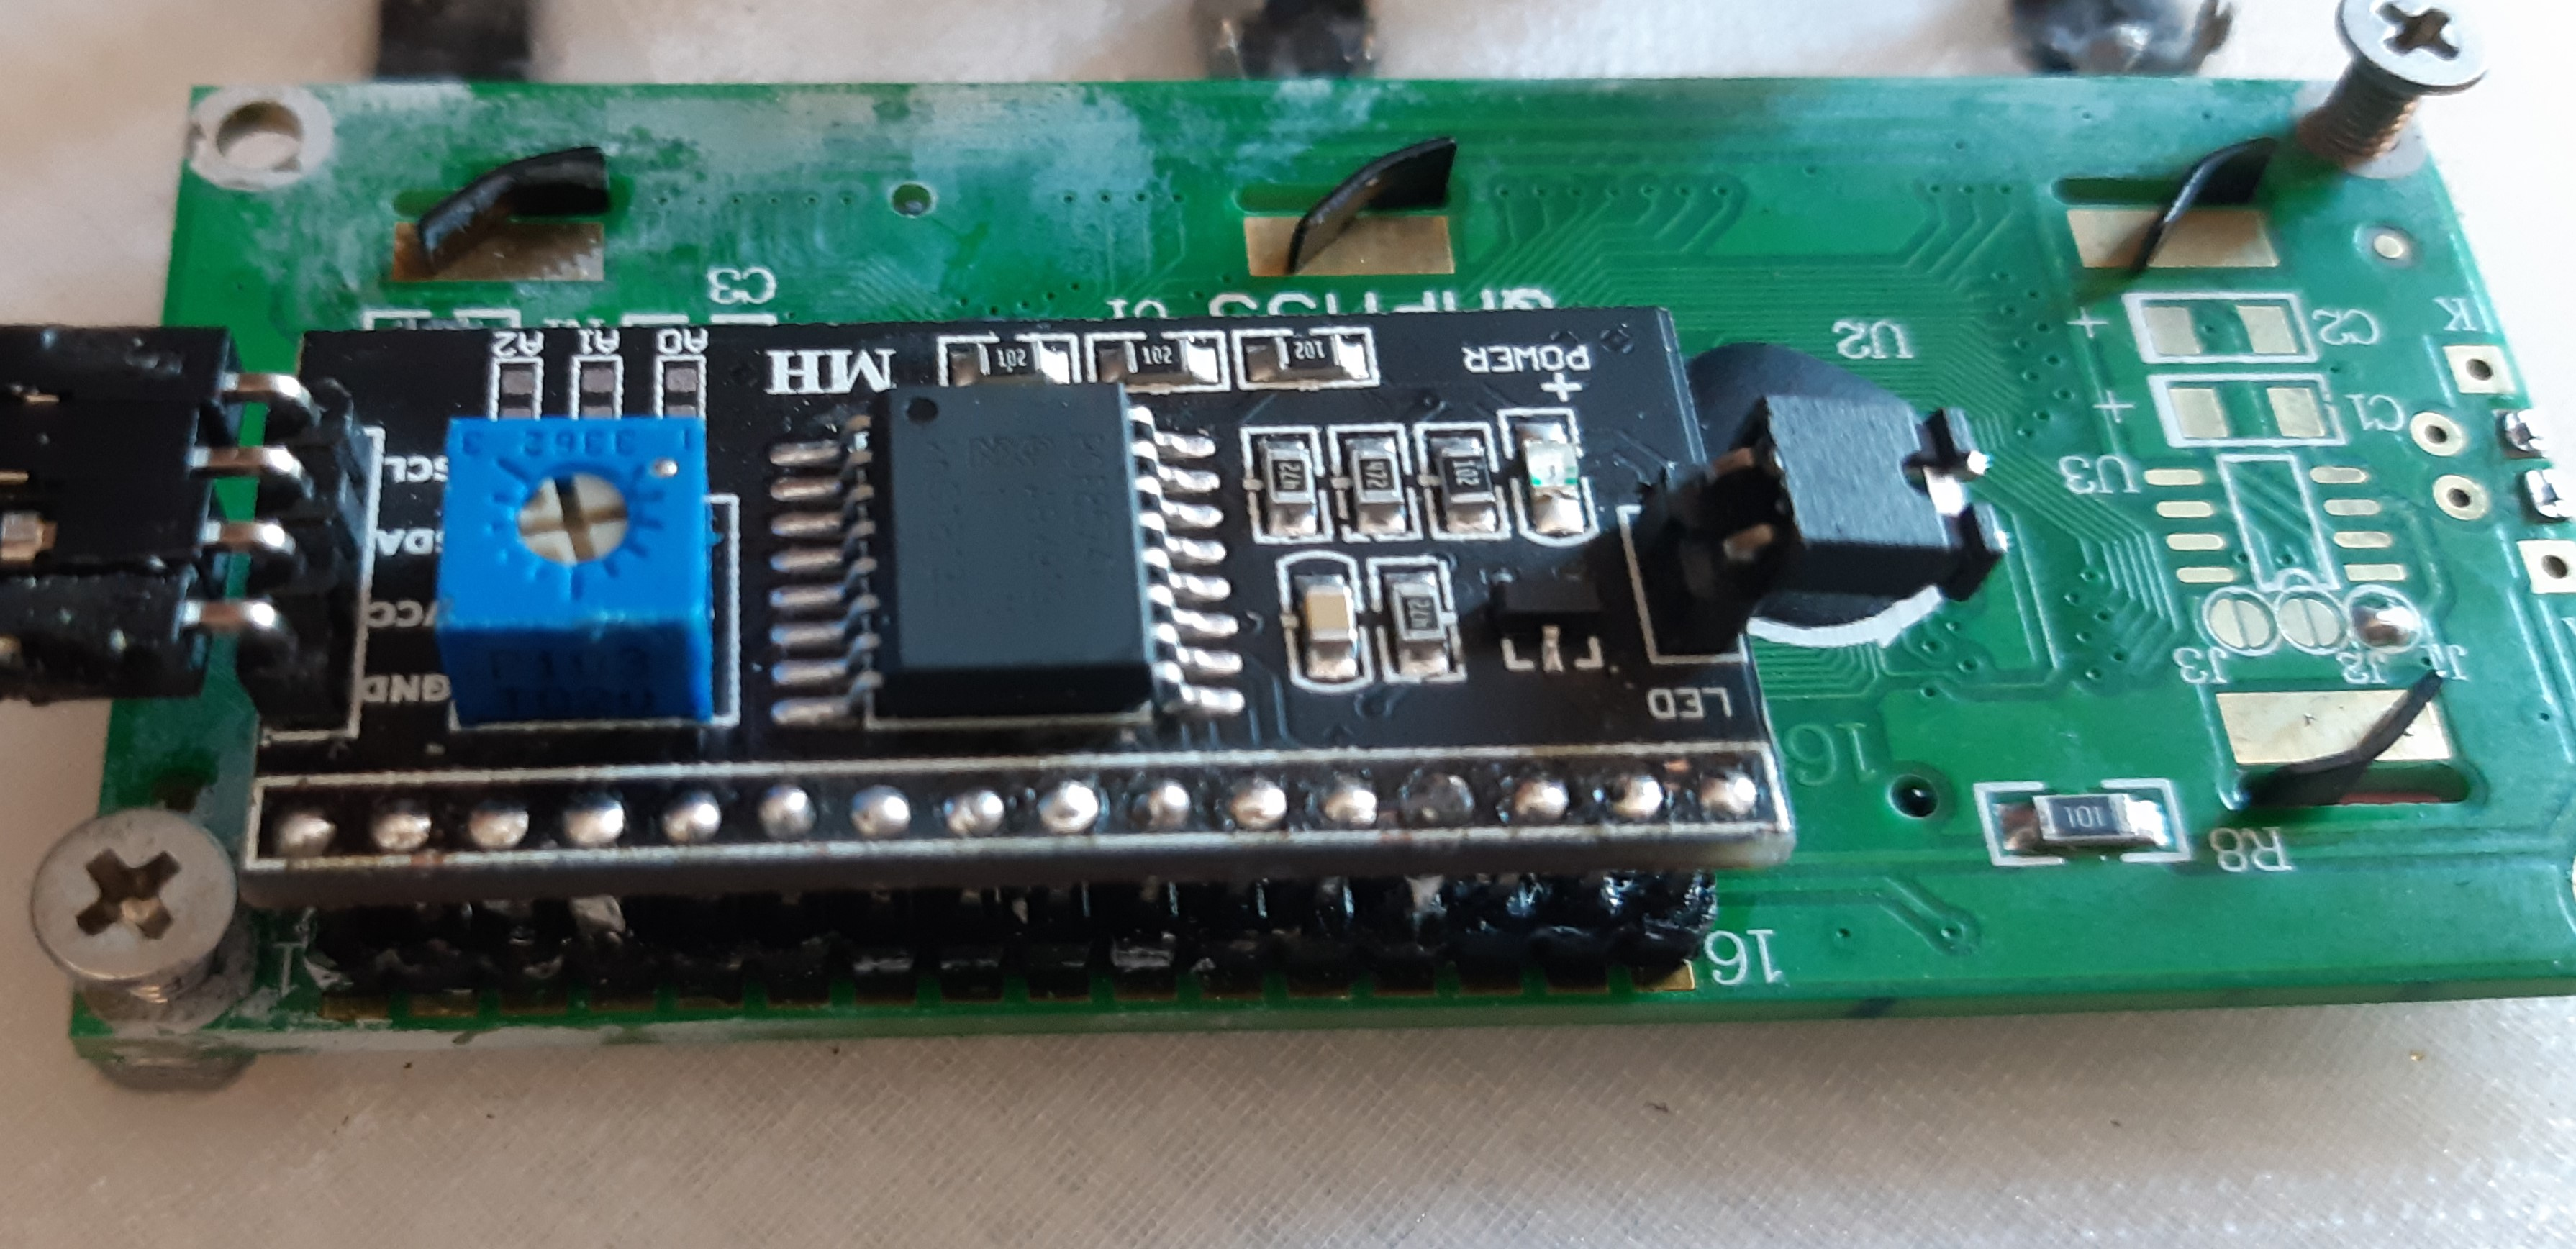
\includegraphics[width=0.6\linewidth]{Images/I2C}
	\footnotesize \\Quelle: eigene Aufnahme
	\caption{Anschluss des I$^2$C-Adapters an das \ac{LCD}-Display}
	\label{fig:I2C}
\end{figure}

In der Tabelle \ref{tab:PINs} sind alle Verbindungen zwischen den einzelnen Komponenten mit dem Arduino aufgelistet. In Abbildung \ref{fig:Layout} ist das enprechende Layout als Zeichnung zu finden. Achten Sie darauf, dass der Arduino während dieser Arbeit vom Stromnetz getrennt ist, um Kurzschlüsse zu vermeiden.

\begin{table}[!hbt]
	\centering
	\begin{tabular}{|r|l|l|l|}
		\hline
		Nummer & Bauteil & Spezifikation & Anschlusspin Arduino \\
		\hline
		1 & I$^2$C-Adapter & GND & GND \\
		 & & SDA & A1 \\
		 & & SCL & A0 \\
		\hline
		2 & \ac{LED}s & Rot & A3 \\
		 & & Gelb & A2\\
		 & & Grün & A1\\
		 & & Blau & A0\\
		\hline
		3 & Taster & Up-Button & 12 \\
		 & & Enter-Button & 13 \\
		\hline	
		4 & CCS811 & WAK & GND \\
		 & & SDA & SDA \\
		 & & SCL & SCL \\
		 & & VCC & 5V \\
		\hline
		5 & Mikro-SD-Adapter & GND & GND \\
		 & & MISO & D11 \\
		 & & MOSI & D10 \\
		 & & SCK & 9 \\
		 & & CS & 8 \\
		 & & VCC & 5V \\
		\hline
	\end{tabular}
	\captionabove{Zuordnung der Pins}
	\label{tab:PINs}
\end{table}

Auch die Vorwiderstände, welche Sie in Tabelle \ref{tab:Widerstände} sehen können, sind essentiell, um eine erfolgreiche Installation zu garantieren.

\begin{table}[!hbt]
	\centering
	\begin{tabular}{|r|l|l|}
		\hline
		Nummer & Bauteil & Vorwiderstand \\
		\hline
		1 & \ac{LED}s & 330$\ohm$ \\
		\hline
		2 & Taster & 2K$\ohm$ \\
		\hline
	\end{tabular}
	\captionabove{Verwendete Vorwiderstände innerhalb der Schaltung}
	\label{tab:Widerstände}
\end{table}

Bevor der Arduino an das Stromnetz geschlossen werden kann, kontrollieren Sie, ob sich eine Mikro-SD-Karte in dem dafür vorgesehenen Adapter befindet. Verbinden Sie anschließend das Gerät mit einer geeigneten Stromquelle. Das Menü öffnet sich und das Gerät ist installiert. Achten Sie darauf, dass der Arduino während einer Messung nicht von der Stromquelle getrennt wird. \\


\chapter{Fazit}
%Fazit - Autor:
\label{Fazit}



\addchap{Verzeichnis verwendeter Abkürzungen und Formelzeichen}

\begin{acronym}%[CSMA/CD + AMP]
	
	\acro{DHBW}{Duale Hochschule Baden-Würtemberg}
	\acro{MOX}{Metalloxid}
	\acro{AD}{Analog-Digital}
	\acro{LCD}{LiquidCrystal Display}
	\acro{PWM}{Pullsweitenmodulation}
	\acro{HDMI}{High Definition Multimedia Interface}
	
\end{acronym}

% ---- Literaturverzeichnis ----------

\bibliography{quellen/ccs811}
										% Einbindung mehrerer Verzeichnisse in einem \bibliography Befehl mit Kommata trennen - keine Leerzeichen nach den Kommata!
\bibliographystyle{alphadin}           	%plain: alphabetisch, unsrt: nach Zitat, alphadin: NameJahr


% -----Ausgabe aller Verzeichnisse ---
\setlength{\parskip}{0.5\baselineskip}
\renewcommand{\indexname}{Sachwortverzeichnis}
\printindex								% Erzeugen des Indexverzeichnises
\addcontentsline{toc}{chapter}{\indexname}
% Version 0.1 vom 31.10.14 - T. Kibler

% Änderungswünsche bitte an T. Kibler melden

% alle Abkürzungen, die in der Arbeit verwendet werden. Nachfolgend sind allgemeine Abkürzungen aufgelistet. Die für die Arbeit spezifischen Abkürzungen sollten innerhalb des Haupttextes aufgeführt werden. Die Alphabetische Sortierung übernimmt Latex.

				% Datei mit allgemeinen Abkürzungen laden
%\renewcommand{\nomname}{Verzeichnis verwendeter %Formelzeichen und Abkürzungen}
%\setlength{\nomlabelwidth}{.20\hsize}
%\renewcommand{\nomlabel}[1]{#1 \dotfill}
%\setlength{\nomitemsep}{-\parsep}
%\printnomenclature						% Erzeugen des Abkürzungsverzeichnises, siehe auch Inhalt der Datei pages/abkuerzungen.tex
%\cleardoublepage
%\renewcommand{\glossaryname}{Glossar}
%\printglossaries
%\cleardoublepage
\listoffigures 							% Erzeugen des Abbildungsverzeichnisses 
\cleardoublepage
\listoftables 							% Erzeugen des Tabellenverzeichnisses
\cleardoublepage

% -----Anhang ------------------------
\appendix
\chapter{Anhang}

\section{Weitere Abbildungen}
%\clearpage
%\pagenumbering{Roman}					% große, römische Seitenzahlen für Anhang, falls gewünscht

\end{document}